% Very simple template for lab reports. Most common packages are already included.
\documentclass[a4paper, 11pt]{article}
\usepackage[utf8]{inputenc} % Change according your file encoding
\usepackage{graphicx}
\usepackage{url}
\usepackage{listings}
\usepackage{float}

%----------------------Definition pour listings------------------------
\lstset{ %
basicstyle=\footnotesize,       % the size of the fonts that are used for the code
%numbers=left,                   % where to put the line-numbers
%numberstyle=\footnotesize,      % the size of the fonts that are used for the line-numbers
%stepnumber=1,                   % the step between two line-numbers. If it's 1 each line
				% will be numbered
%numbersep=5pt,                  % how far the line-numbers are from the code
%backgroundcolor=\color{white},  % choose the background color. You must add \usepackage{color}
showspaces=false,               % show spaces adding particular underscores
showstringspaces=false,         % underline spaces within strings
showtabs=false,                 % show tabs within strings adding particular underscores
frame=single,                    % adds a frame around the code
tabsize=2,                        % sets default tabsize to 2 spaces
captionpos=b,                   % sets the caption-position to bottom
breaklines=true,                % sets automatic line breaking
breakatwhitespace=false,        % sets if automatic breaks should only happen at whitespace
		 % show the filename of files included with \lstinputlisting;
				% also try caption instead of title
escapeinside={\%*}{*)},         % if you want to add a comment within your code
morekeywords={*,...}            % if you want to add more keywords to the set
}

%opening
\title{Report: Routy, a small routing protocol}
\author{Alexandre Tamborrino}
\date{\today{}}

\begin{document}

\maketitle

\section{Introduction}

During this seminar we have implemented in Erlang a routing protocol based on the well-known link-state routing protocol.

In our implementation, a router can broadcast link-state messages to all their gateways (neighbor routers) in order to tell them what are all its gateways. These neighbor routers process the link-state message (save the information) and broadcast it to all their own gateways. Thus, each link-state message of a router goes through the whole network, therefore all the routers know what are the gateways of the router who has initially send the link-state message. If each router does this, all routers will have a complete map of the network.

Then each router can compute a routing table to know where to route a message that has to go to a specific destination. The processing of the table uses the Dijkstra algorithm to find shortest paths in the network. Thus, messages can be routed effectively. We will see the limitations of this implementation in the conclusion.

\section{Main problems and solutions}

As I did not have the "very helpful code skeleton file" when I implemented Routy, I encounter some difficulties about how to solve things in a functional programming way.
For example, in the Dijkstra algorithm, I was wondering how to iterate over a list updating another list at each iteration. As variables are immutable, I was wondering how to update the list in a way that each iteration uses the updated version of the previous iteration. Then, I look to the lists:foldl/3 function and see what I had to do. Here is the code (part of the Dijkstra algorithm):
\begin{lstlisting}[language=erlang]
NewSortedList = lists:foldl(fun(El,SortedList) ->
		    update(El,L+1,Gateway,SortedList)
		    end, T, Reachables);
\end{lstlisting}

Concerning the history data structure, I have used an Erlang \textit{dict} in order to gain performance. Indeed, this data structure is contained in each router of the network and has N entry (N is the number of routers in the whole network). In order to scale, the hist:update function has to be fast (\textit{dict} has a better complexity than a classic list of tuples in O(N)).


\section{Evaluation}

In order to test my implementation, I set up 3 different Erlang nodes (VM), each representing a country. I wrote an Erlang test module that starts several routers in each country, makes the connections between routers, then broadcasts and updates each router. Figure \ref{fig:map} shows the map of the test network.
\begin{figure}[H]
  \begin{center}
    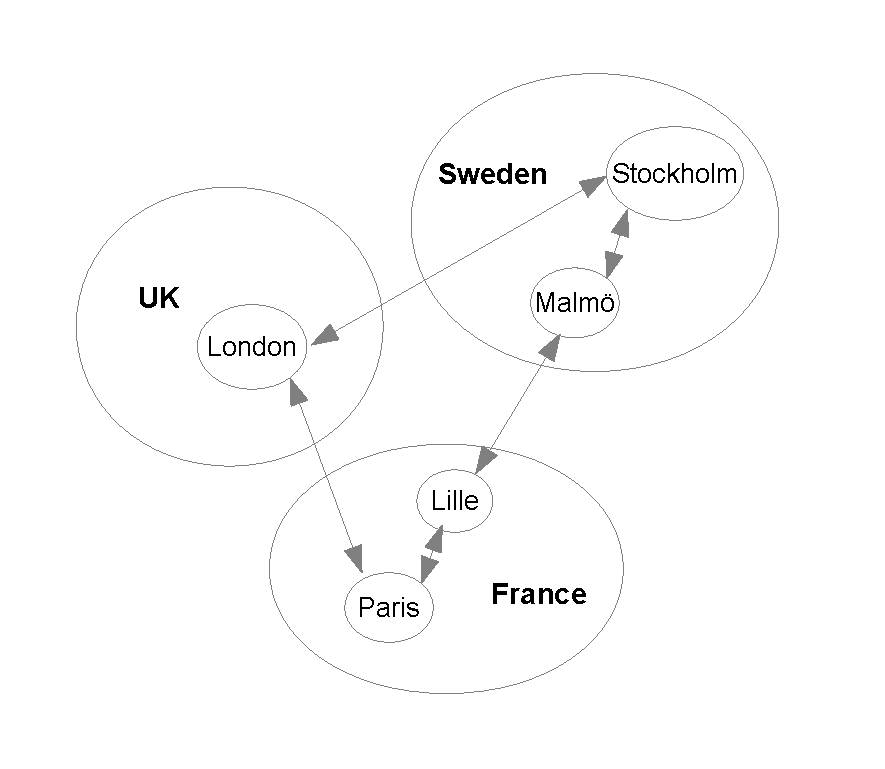
\includegraphics{map.pdf}
    \caption{Network map for testing}
    \label{fig:map}
  \end{center}
\end{figure}
Then I have tested to route a message from Paris to Stockholm. Here is the result of io:format on the different shells:
\begin{lstlisting}
On "France Node":
	$> paris ! {send,stockholm,"Hello Stockholm, this is Paris."}.
	paris: routing message (Hello Stockholm, this is Paris.)

On "UK Node":
	london: routing message (Hello Stockholm, this is Paris.)

On "Sweden Node":
	stockholm: received message Hello Stockholm, this is Paris.
\end{lstlisting}
We see that the message has been correctly routed using the shortest path between Paris and Stockholm.

Now, I shutdown the UK Node. Paris and Stockholm receive the exit message ("DOWN") of London. Then, I broadcast and update Paris and Stockholm. I re-try to route a message from Paris to Stockholm:
\begin{lstlisting}
On "France Node":
	$> paris ! {send,stockholm,"Hello Stockholm, this is Paris."}.
	paris: routing message (Hello Stockholm, this is Paris.)
	lille: routing message (Hello Stockholm, this is Paris.)

On "Sweden Node":
	malmo: routing message (Hello Stockholm, this is Paris.)
	stockholm: received message Hello Stockholm, this is Paris.
\end{lstlisting}
The message is correctly routed in spite of the fact that UK has crashed, therefore our protocol is fault-tolerant.

\section{Conclusions}

During this seminar I have understood and implemented a routing protocol based on link-state. Fault-tolerancy is handled (if some routers crash, messages are still successfully routed). Scaling is limited because each router builds a routing table for the entire network. This can be problematic in very large network. It would be interesting to implement \textit{default routes} to overcome this issue.

\end{document}
